\documentclass{article}
\usepackage{graphicx}
\usepackage[margin=1.5cm]{geometry}
\usepackage{amsmath}

\begin{document}
\twocolumn

\title{Quiz 3: Digital Signal Processing}
\author{Prof. Jordan C. Hanson}

\maketitle
\small

\begin{enumerate}
\item According to the \textbf{Doppler effect}, the frequency of electromagnetic waves reflecting from a moving target will shift in proportion to the velocity of the target.  Let $f_t$ represent the transmitted frequency, $f_r$ represent the reflected frequency, and $f_d = f_r - f_t$.  To first order in $v/c$, 
\begin{equation}
f_d \approx 2 v \frac{f_t}{c}
\end{equation}
(a) Suppose the relative velocity $v$ between our craft and the enemy fighter is $v \approx 300$ m s$^{-1}$, and our radar operates at 1 GHz.  What is the Doppler shift, $f_d$? (b) Given that our receiver has to resolve the difference between $f_t = 1$ GHz and $f_d$, for how long do we have to record the reflected waveform? That is, how do we achieve the required frequency resolution? (c) If we sample at 2 GHz, how many samples would be in the waveform?  Is this practical? \\ \vspace{3cm}
\end{enumerate}

\begin{figure}
\centering
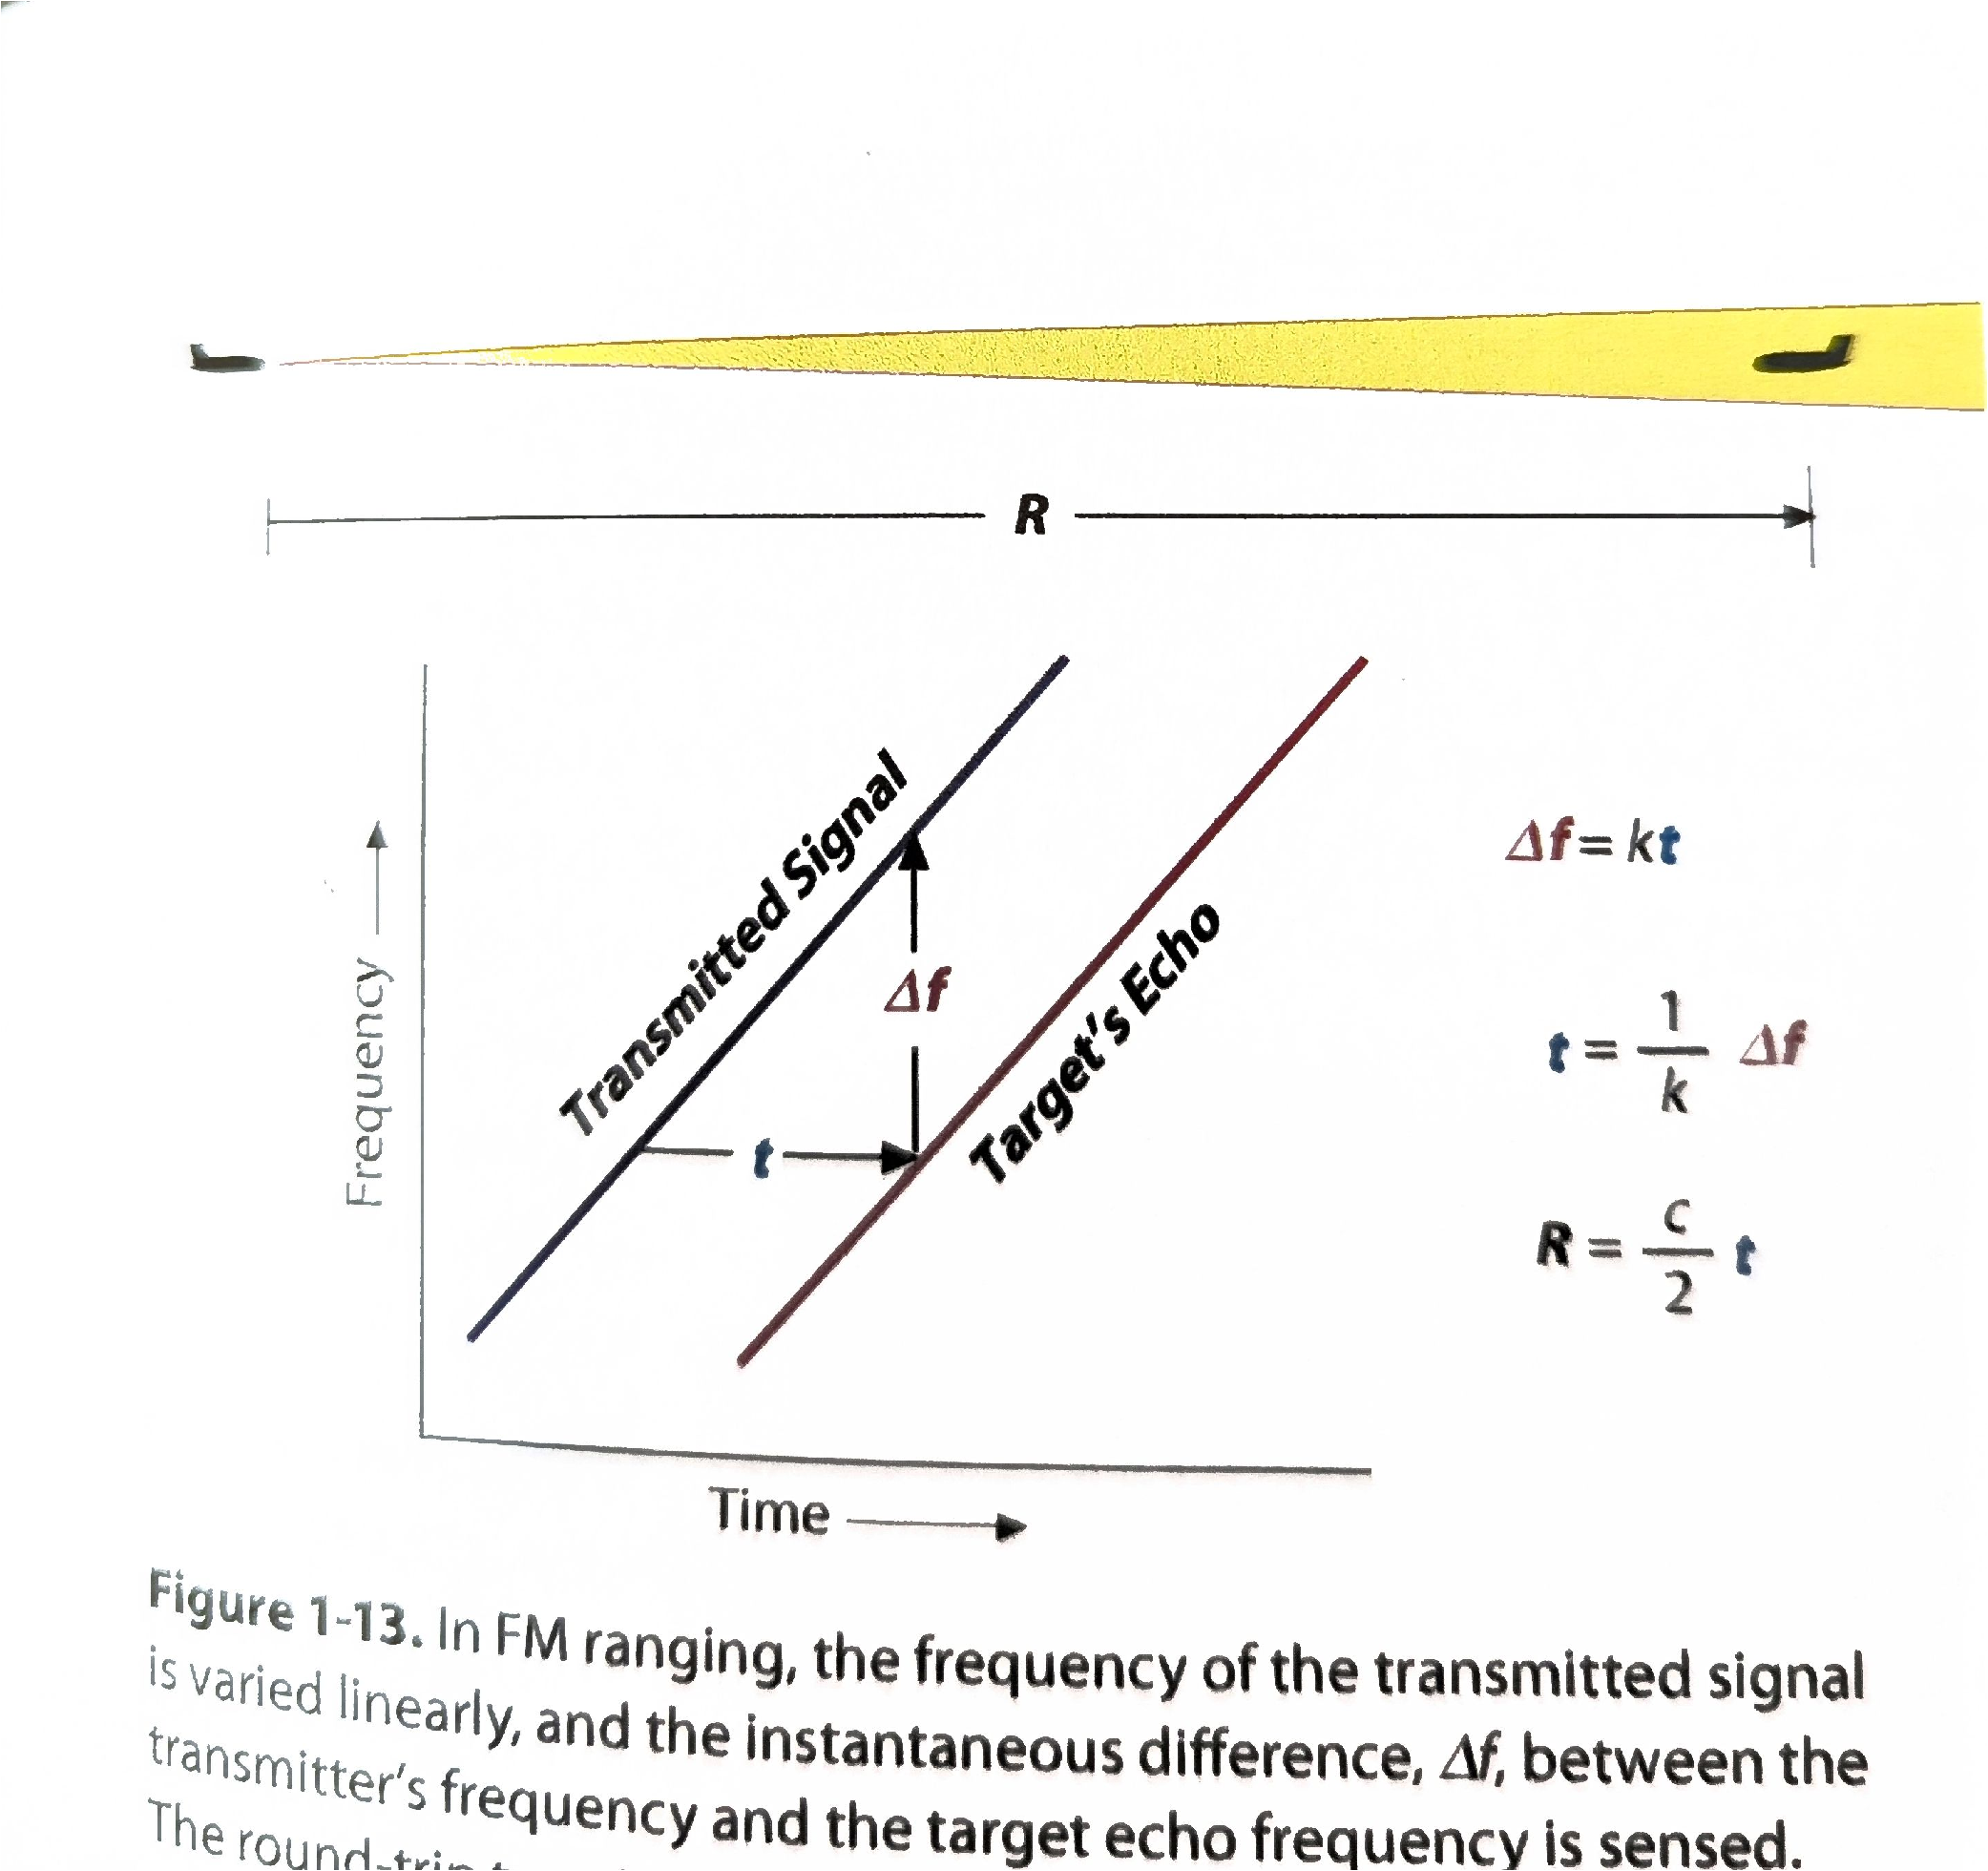
\includegraphics[width=0.5\textwidth,trim=0cm 6cm 0cm 0cm,clip=true]{radar.pdf}
\caption{\label{fig:1} In a basic chirping RF signal scheme used to detect enemy aircraft, a transmitted RF signal is linearly chirped.  Information in the radar echo can be used to find the range, $R$.}
\end{figure}

\end{document}
